\documentclass{article}

% --------------- PAQUETES ---------------
\usepackage[utf8]{inputenc}
\usepackage[spanish]{babel}
\usepackage{amsmath, amssymb}
\usepackage{physics}
\usepackage{siunitx}
\usepackage{xcolor}
\usepackage{tcolorbox}
\usepackage{cancel}
\usepackage{multicol}
\usepackage[
    top=2.5cm,
    bottom=2.5cm,
    left=3.3cm,
    right=3.3cm
]{geometry}
\usepackage{tikz}
\usetikzlibrary{angles, quotes}
\usepackage{float}
\usepackage{hyperref}  


% --------------- COLORES PERSONALIZADOS ---------------
\definecolor{sectionColor}{HTML}{2240f0}
\definecolor{definicionColor}{HTML}{2240f0}
\definecolor{titleColor}{HTML}{ff0000}
\definecolor{exerciceColor}{HTML}{00d5ff}

% --------------- COMANDOS PERSONALIZADOS ---------------
\newcommand{\newsection}[1]{
    \section{\centering \color{sectionColor} \bl{#1}}
}

\newcommand{\newsubsection}[1]{
    \subsection{\color{sectionColor} #1}
}

\newcommand{\newtitle}[1]{
    \vspace{0.5cm}
    \noindent{\large \color{titleColor} \textbf{#1}}\\[0.2cm]
}

\newcommand{\newex}[1]{
    \vspace{0.5cm}
    \noindent{\large \color{exerciceColor} \textbf{#1}}\\[0.2cm]
}

\newcommand{\bl}[1]{\textbf{#1}}


\newtcolorbox{definicionbox}{
    colback=white,      % fondo blanco
    colframe=blue,     % borde negro
    boxrule=2pt,      % grosor del borde
    arc=0pt,            % sin esquinas redondeadas
    left=10pt, right=8pt, top=8pt, bottom=10pt, % margen interno
}

\newcommand{\definicion}[1]{%
    \vspace{0.5cm}
    \begin{definicionbox}
        #1
    \end{definicionbox}
    \vspace{0.5cm}
}

% --------------- ENCABEZADO ---------------
\title{Apunte Física 1}
\author{Luca Di Bene}
\date{\today}

% --------------- DOCUMENTO ---------------
\begin{document}

    \maketitle
    \tableofcontents
    \newpage

% ------------------- SECCIÓN 1 -------------------
    \newsection{Unidades, Cantidades Físicas y Vectores}

    % ----------------- NUEVA SUBSECCIÓN -----------------

    \newsubsection{La Física}

    \par La Física es una \bl{ciencia experimental} que busca explicar fenómenos naturales a través de la observación y la experimentación. Los físicos formulan teorías mediante \bl{modelos ideales, leyes y principios físicos}. Estas teorías se desarrollan con creatividad, pruebas y observaciones, como hizo Galileo al investigar la caída de los cuerpos.

    \newtitle{Resolución de problemas}

    \par Resolver problemas permite aplicar conceptos. El proceso incluye:

    \begin{enumerate}
        \item \underline{Identificar conceptos}: Elegir qué principios físicos son relevantes.
        \item \underline{Plantear el problema}: Traducirlo a ecuaciones.
        \item \underline{Ejecutar la solución}: Sustituir valores y hacer cálculos.
        \item \underline{Evaluar la respuesta}: Verificar si tiene sentido físico.
    \end{enumerate} 

    \begin{multicols}{2}

    \begin{center}
    \begin{minipage}[t]{0.60\textwidth}
    \newtitle{Modelos idealizados}
        \smallskip

        \par En física, simplificamos los sistemas complejos creando \bl{modelos idealizados} que omiten detalles irrelevantes. Estos modelos son válidos dentro de ciertos límites, como el modelo de caída libre de Galileo que omite la resistencia del aire.
        \par La física describe el mundo mediante \bl{modelos matemáticos}, que permiten hacer predicciones razonables sobre el comportamiento de los sistemas.

    \end{minipage}

    \hfill
    \columnbreak
    
    \begin{minipage}[t]{0.35\textwidth}

        \bigskip
        \par Para simplificar el análisis de a) una pelota de béisbol lanzada al aire, usamos b) un modelo idealizado.
        \smallskip
        \par a) Una pelota real lanzada al aire.
        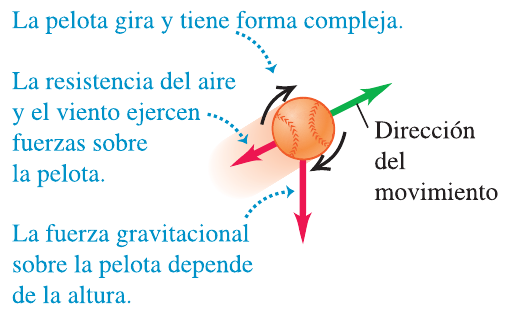
\includegraphics[width=\linewidth]{img/1.1-1.png}

        \par b) Un modelo idealizado de una pelota real lanzada al aire.
        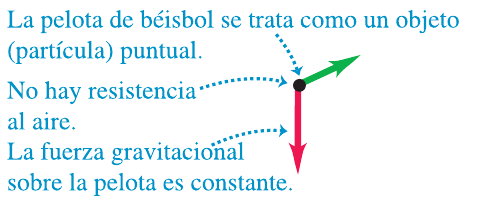
\includegraphics[width=\linewidth]{img/1.1-2.png}

    \end{minipage}
    \end{center}

    \end{multicols}

    % ----------------- NUEVA SUBSECCIÓN -----------------

    \newsubsection{Mediciones, magnitudes y unidades}

    \newtitle{Magnitudes físicas y unidades}

    \par Las \bl{magnitudes físicas} son propiedades medibles como masa, longitud o tiempo. El \bl{Sistema Internacional (SI)} define unidades básicas:

    \begin{itemize}
        \item \bl{Longitud}: metro (\bl{m})
        \item \bl{Masa}: kilogramo (\bl{kg})
        \item \bl{Tiempo}: segundo (\bl{s})
    \end{itemize}

    \par Las unidades derivadas (como velocidad o energía) se forman combinando unidades básicas.

    \newtitle{Conversión de unidades}

    \begin{enumerate}
        \item \underline{Identificar}: qué unidades hay que convertir.
        \item \underline{Plantear/Ejecutar}: usar factores de conversión.
        \item \underline{Evaluar}: comprobar que tenga sentido.
    \end{enumerate}

    \[
        3\cancel{\text{min}} \times \frac{60s}{1\cancel{\text{min}}} = 180s
    \]

    \newtitle{Incertidumbre}

    \par Toda medición tiene \bl{incertidumbre}, que refleja el límite del instrumento. Se expresa como:

    \[
        \text{valor medido} \pm \text{error}
    \]

% ------------------- NUEVA SUBSECCIÓN -------------------
    \newsubsection{Vectores y Suma de Vectores}

    \newtitle{Cantidades escalares y vectoriales}

    \par En física, algunas cantidades pueden ser descritas solo con un número y una unidad (\bl{escalares}), como el tiempo, la masa o la temperatura. Otras, en cambio, requieren una dirección además de una magnitud (\bl{vectores}). La velocidad y la fuerza son ejemplos típicos: no basta con saber cuánto valen, también es esencial saber \bl{hacia dónde} actúan o se mueven.
    \par Un vector se representa con una \bl{flecha}. La \bl{longitud} indica la magnitud y la \bl{orientación} muestra su dirección. Por convención, los vectores se nombran con letras negritas y con una \bl{flecha arriba}, como \(\vec{A}\), para diferenciarlos de los escalares.

    \begin{figure}[H]
        \centering
        \shorthandoff{>}
        \begin{tikzpicture}[scale=2]
            \draw[->] (0,0) -- (2,1) node[midway, above] {$\vec{A}$};
        \end{tikzpicture}
    \end{figure}

    \definicion{
        \centering
        \par \underline{Magnitud}: A o \(\lvert \vec{A} \rvert\) indican cuánto mide \(\vec{A}\), sin dirección.
        }

    \begin{multicols}{2}
        \centering

        \begin{minipage}[t]{0.6\textwidth}

            \par Dos vectores son \bl{iguales} si tienen la misma \bl{magnitud} y \bl{dirección}, aunque estén ubicados en lugares diferentes.

        \end{minipage}
        \hfill
        \columnbreak
        \begin{minipage}[t]{0.3\textwidth}

            \begin{figure}[H]
                \centering
                \shorthandoff{>}
                \begin{tikzpicture}[scale=1.2]
                    \draw[->, blue] (0,0) -- (1,1) node[midway, above] {$\vec{A}$};
                    \draw[->, red] (1,0) -- (2,1) node[midway, above] {$\vec{B}$};
                \end{tikzpicture}
                \shorthandon{>}
            \end{figure}

        \end{minipage}
        
    \end{multicols}

    \begin{multicols}{2}
        \centering

        \begin{minipage}[t]{0.6\textwidth}

            \par Un vector \bl{opuesto} tiene igual magnitud pero direción contraria, lo llamamos el negativo del vector original.

        \end{minipage}
        \hfill
        \columnbreak
        \begin{minipage}[t]{0.3\textwidth}

            \begin{figure}[H]
                \centering
                \shorthandoff{>}
                \begin{tikzpicture}[scale=1.2]
                    \draw[->, blue] (0,0) -- (1,1) node[midway, above] {$\vec{A}$};
                    \draw[->, red] (2,1) -- (1,0) node[midway, below, right] {$\vec{B}=-\vec{A}$};
                \end{tikzpicture}
                \shorthandon{>}
            \end{figure}

        \end{minipage}
        
    \end{multicols}

    \par \underline{Suma de vectores}: Para sumar vectores gráficamente, se usa el metodo "\bl{cola con punta}": se coloca el origen del segundo vector en el extremo del primero.
    \begin{figure}[H]
        \centering
        \shorthandoff{>}
        \begin{tikzpicture}[scale=1]
            \draw[->, gray] (0,0) -- (3,1) node[midway, below] {$\vec{A}$};
            \draw[->, gray] (3,1) -- (2,3) node[midway,right] {$\vec{B}$};
            \draw[->, blue] (0,0) -- (2,3) node[midway, above, left] {$\vec{A}+\vec{B}$};
        \end{tikzpicture}
        \shorthandon{>}
    \end{figure}

    \par No importa el orden en que sumes los vectores, siempre da el mismo resultado.
    \[ \vec{A}+\vec{B}=\vec{B}+\vec{A} \]

    \par \underline{Resta de vectores}: Restar vectores significa sumar el \bl{opuesto}. Si queremos calcular \(\vec{A}-\vec{B}\), lo que realmente hacemos es sumar \(\vec{A}\) con el negativo de \(\vec{B}\).
    \[ \vec{A}-\vec{B}=\vec{A}+(-\vec{B}) \]

    % ---------------- NUEVA SUBSECCIÓN ----------------

    \newsubsection{Componentes de vectores}

    \par Cuando sumamos vectores, muchas veces es más fácil descomponerlos en \bl{componentes} sobre un sistema de ejes perpendiculares.
    \par Un vector \(\vec{A}\) puede descomponerse en dos vectores: uno paralelo al eje x (\(\vec{A}_x\)) y otro paralelo al eje y (\(\vec{A}_y\)). La suma de estos dos vectores da como resultado el vector original: \(\vec{A}=\vec{A}_x+\vec{A}_y\).

    \begin{figure}[H]
        \centering
        \shorthandoff{>}
        \begin{tikzpicture}[scale=1.2]
            \draw[->, black] (0,0) -- (3,0) node[below] {$x$};
            \draw[->, black] (0,0) -- (0,3) node[left] {$y$};

            \draw[->, blue] (0,0) -- (1,2) node[midway, above, left] {$\vec{A}$};
            \draw[->, red] (0,0) -- (1,0) node[midway, below] {$\vec{A}_x$};
            \draw[->, green] (0,0) -- (0,2) node[midway, above, left] {$\vec{A}_y$};
            \draw[-, dashed, gray] (1,0) -- (1,2);
            \draw[-, dashed, gray] (0,2) -- (1,2);

            % angle
            \draw[->, black] (0.5,0) .. controls (0.5,0.4) and (0.3,0.5) ..  (0.25,0.5) node[midway, above, right] {$\theta$};

        \end{tikzpicture}
        \shorthandon{>}
    \end{figure}

    \par Podemos calcular la magnitud de las componentes de $\vec{A}$ si conocemos la magnitud A y su dirección. Describimos la direccion de un vector como el angulo $\theta$ formado por le eje x positivo con el vector en sentido anti horario. Entonces por definición de trigonométricas:
    \[ \lvert \vec{A}_x \rvert = \lvert \vec{A} \rvert \cos \theta \]
    \[ \lvert \vec{A}_y \rvert = \lvert \vec{A} \rvert \sin \theta \]

\newsection{Movimiento en dos o en tres dimensiones}

% ------------------- SECCIÓN 2 -------------------

\newsection{Leyes del movimiento de Newton}

\par En los dos capítulos anteriores estudiamos la cinemática, el lenguaje para describir el movimiento. Ahora estamos en condiciones de pensar en qué hace que los cuerpos se muevan como lo hacen.

\par En este capítulo usaremos dos conceptos nuevos, la fuerza y la masa, para analizar los principios de la dinámica, los cuales están establecidos en solo tres leyes que fueron claramente enunciadas por Sir Isaac Newton:

\begin{itemize}
    \item Primera ley (ley de la inercia): Si la fuerza neta sobre un cuerpo es cero, su movimiento no cambia.
    \item Segunda ley: Relaciona la fuerza con la aceleración cuando la fuerza neta no es cero.
    \item Tercera ley: Es una relación entre las fuerzas que ejercen dos cuerpos que interactúan entre sí.
\end{itemize}

\par Las leyes de Newton no son producto de deducciones matemáticas, sino una síntesis que los físicos han descubierto al realizar un sinnúmero de experimentos con cuerpos en movimiento.

    % ---------------- NUEVA SUBSECCIÓN ----------------

    \newsubsection{Fuerza e interacciones}

        \par En la vida cotidiana hablamos de fuerza como un empujón o un tirón. En física, una fuerza se define mejor como una interacción entre dos cuerpos o entre un cuerpo y su entorno. Esta interacción tiene dirección y magnitud, por lo que se representa como un vector.

    \newtitle{Fuerzas de contacto}

        \par Son fuerzas que requieren interacción directa entre cuerpos. Se distinguen principalmente tres tipos:

        \begin{itemize}
            \item \underline{Fuerza normal}: Es la fuerza ejercida por una superficie sobre un objeto en contacto con ella. Siempre actúa perpendicular a la superficie.
            \item \underline{Fuerza de fricción}: También es ejercida por una superficie, pero actúa paralela a ella y en dirección opuesta al movimiento relativo entre el objeto y la superficie.
            \item \underline{Fuerza de tensión}: Es la fuerza transmitida por cuerdas, cables o cordeles estirados. Actúa a lo largo del cordel y en la dirección de la tracción, como cuando se tira de una cuerda.
        \end{itemize}

        \begin{multicols}{3}
            \centering
            \begin{figure}[H]
                \centering
                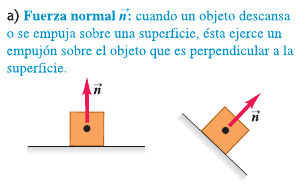
\includegraphics[scale=0.6]{img/2.1-1.png}
                \caption{Fuerza normal}
                \label{fig:Fuerza normal}
            \end{figure}

            \columnbreak

            \begin{figure}[H]
                \centering
                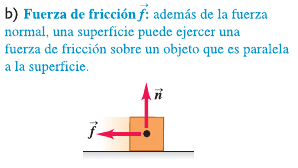
\includegraphics[scale=0.6]{img/2.1-2.png}
                \caption{Fuerza de fricción}
                \label{fig:Fuerza de fricción}
            \end{figure}

            \columnbreak

            \begin{figure}[H]
                \centering
                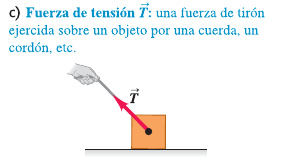
\includegraphics[scale=0.6]{img/2.1-3.png}
                \caption{Fuerza de tensión}
                \label{fig:Fuerza de tension}
            \end{figure}

        \end{multicols}

    \newtitle{Fuerzas a distancia}
        \par Estás actuar sin contacto física Ejemplos comunes son la gravedad, el magnetismo y las fuerzas eléctricas. La fuerza gravitatoria que la tierra ejerce sobre un objetto se llama \bl{peso}.
        \begin{figure}[H]
            \centering
            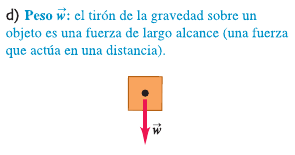
\includegraphics[scale=0.8]{img/2.1-4.png}
            \caption{Fuerza a distancia}
            \label{fig:Fuerza a distancia}
        \end{figure}

    \newtitle{Medición de fuerzas}

        \par La magnitud de una fuerza se mide en "newtons", que se abrevia N. (Daremos una definición precisa del newton más adelante) Un instrumento tipico para medirla es la \bl{balanza de resorte} que aprovecha la relación entre estiramento de un resorte y la fuerza aplicada.

    \newtitle{Superposición de fuerzas}

        \par Cuando varias fuerzas actúan sobre un cuerpo, su efecto combinado es igual al de una única fuerza resultante obtenida mediante la suma vectorial de todas ellas. Esto se conoce como el Principio de superposición. La fuerza neta o resultante total sobre un cuerpo es, la suma vectorial de todas las fuerzas que actúan sobre él. Se denota:
        
        \[\vec{R} = \sum \vec{F}\]

        \par Cada fuerza puede descomponerse en componentes vectoriales, entonces la fuerza neta tambien:

        \[\vec{R_x} = \sum \vec{F_x} \quad , \quad \vec{R_y} = \sum \vec{F_y}\]

    \newsubsection{Primera ley de Newton}

    \definicion{
        \par \color{blue}\underline{\bl{Primera ley}}\color{black}: Todo cuerpo persevera en su estado de reposo o movimiento uniforme y rectilíneo a no ser que sea obligado a cambiar su estado por fuerzas impresas sobre él. 
    }

    \par En esta ley se introduce el concerto de \bl{inercia}, que es la resistencia de un cuerpo a cambiar su estado de movimiento.
    \par Esta ley rompe con la idea aristotélica de que se necesita una fu constante para mantener el movimiento. Newton muestra que en r lo que se necesita es una fuerza para cambiar el movimiento.
    \par Si empujás una caja y después dejas de hacerlo, eventualmente se detiene. No porque "el movimiento se gasta", sino porque existen fuerzas Como la fricción y el rozamiento con el aire que actúan en sentido Contrario al movimiento y Provocan que se frene.

    \newtitle{Marcos de referencia inerciales}

    \par Un \bl{marco de referencia} es un sistema desde el cual se observa y describe el movimiento de los cuerpos.
    \par Un \bl{marco de referencia inercial} es aquel en el cual se cumple la Primera Ley de Newton, es decir que si un objeto cambia su Velocidad, entonces desde el marco se ve una fuerza actuando.

    \newsubsection{Segunda ley de Newton}

    \par Podemos ver que existe una relación proporcional entre la fuerza y la aceleración. Si empujamos una caja con una fuerza neta constante, la caja tendra una acelarión constante igual a $a=\vec{a}$.
    \par Si utilizamos una balanza de resorte Para aplicar una fuerza $\vec{F_1}$ obtenemos una aceleración $\vec{a}$, para $2\vec{F_1}$, obtenemos $2\vec{a}$ y para $\frac{1}{2}\vec{F_1}$ $\frac{1}{2}\vec{a}$. Muchos experimentos semejantes muestran que para un cuerpo dado, la magnitud de la aceleración es directamente propor-cional a la magnitud de la fuerza neta que actúa sobre él.

    \newtitle{Masa y fuerza}

   \par Nuestros resultados indican que para un cuerpo dado, el cociente $\left\lvert \Sigma \vec{F}\right\rvert $ entre $\left\lvert \vec{a} \right\rvert $ es constante. Llamamos a este cocient \bl{masa inercial} del cuerpo y la denotamos con \bl{m}. Es decir,

    \[ m = \frac{\lvert \Sigma \vec{F}\rvert }{\lvert \vec{a} \rvert } \quad,\quad
    \lvert \Sigma \vec{F} \rvert = m \lvert \vec{a} \rvert \quad o \quad
    \lvert \vec{a} \rvert = \frac{\lvert \Sigma \vec{F}\rvert }{m}\]

    \par La ultima de las ecuaciones indica que cuanto mayor sea su masa, más se "resiste" un cuerpo a ser acelerado.
    \par La unidad de masa en el SI es el kilogramo. Podemos usar este Kilogramo para definir el newton:

    \definicion{
        \par Un Newton es la cantidad de fuerza neta que proporciona una aceleración de 1 metro por segundo al cuadrado a un cuerpo con masa de 1 Kilograma.
    }

    \par Por la forma en que definimos el newton, está relacionado con las unidades de masa, longitud y tiempo.

    \[ 1 \text{N} = 1 \text{kg} \cdot \text{m/s}^2 \]

    \begin{table}[H]
        \centering
        \begin{tabular}{|c|c|c|c|}
            \hline
            Sistema de unidades & Fuerza & Masa & Aceleración \\
            \hline
            SI & Newton(N) & Kg & $m/s^2$ \\
            \hline
            cgs & dina(din) & g & $cm/s^2$ \\
            \hline
            Imperial & libra(lb) & slug & $ft/s^2$ \\
            \hline
        \end{tabular}
    \end{table}

    \newtitle{Enunciado de la segunda ley de Newton}

    \definicion{
        \par \color{blue}\underline{\bl{Segunda ley}}\color{black}: si una fuerza externa neta actúa sobre un Cuerpo, éste se acelera. La dirección de aceleración es la mis ma que la dirección de la fuerza neta. El vector de fuerza neta es igual a la masa del cuerpo multiplicada por su aceleración. En símbolos: 

        \[\Sigma \vec{F} = m \vec{a}\]
    }

    \par La segunda ley de Newton es una ley fundamental de la naturaleza, la relación básica entre fuerza y movimiento, Casa todo el resto del capítulo, y todo el que sigue, se dedica a aprender a aplicar este principio en diversas situaciones.

    \newtitle{Uso de la segunda ley de Newton}

    \par Hay al menos cuatro aspectos de la segundo ley de Newton que Merecen atención especial:

    \begin{enumerate}
        \item \bl{Forma de uso}: La segunda lev de Newton es una ecuación Vectorial, Pero normalmente se usa descompuesta por componentes:
        \[\Sigma \vec{F_x} = m \vec{a_x} \quad , \quad \Sigma \vec{F_y} = m \vec{a_y}\]

        \item \bl{Fuerzas externes}: La ley se refiere únicamente a Fuerzas externas es decir, ejercidas sobre el cuerpo desde otros cuerpos o el entorno. Un cuerpo no puede moverse por una fuerza que el mismo genera.
        \item \bl{Masa constante}: Estas ecuaciones solo son válidas si las masa no cambia. En casos donde la masa varía (cohete que pierda combustible) se necesita un tratamiento especial.
        \item \bl{Marcos de referencia inenciales}: La ley solo se aplica en marcos de referencia inerciales. No vale en marcos acelerados, como dentro de un auto que arranca.
    \end{enumerate}

    \newsubsection{Masa y Peso}

    \begin{multicols}{2}
        \begin{minipage}[t]{0.7\textwidth}
            \par Es común usar incorrecta e indistintamente los términos \bl{masa} y \bl{peso} en las conversaciones cotidianas. Es absolutamente indispensable entender claramente las diferencias entre estas dos cantidades físicas.

            \par La \bl{masa} Caracteriza las Propiedades inerciales de un cuerpo. A mayor masa, se necesitará más fuerza Para causar una aceleración dada.

            \par El \bl{peso}, en cambio, es una fuerza ejercida sobre un cuerpo por la atracción de la Tierra.

            \par Para entender la relación entre masa y peso, note que un cuerpo en caída libre tiene una aceleración igual a gy, Por la segunda ley de Newton, una fuerza produce esa aceleración. Si un cuerpo de masam cae con una aceleración $\vec{g}$ con $ \lvert \vec{g} \rvert = 9.8 \text{m/s}^2 $, entonces: $\vec{w} = m \vec{g}$
        \end{minipage}

        \columnbreak

        \begin{minipage}[t]{0.7\textwidth}
            \begin{figure}[H]
                \centering
                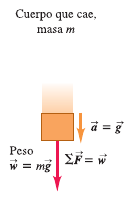
\includegraphics[scale=1]{img/2.4-1.png}
            \end{figure}
        \end{minipage}
    \end{multicols}

    \newtitle{Variación de g con la ubicación}

    \par En la tierra se usa $g \approx 9,80 m/s^2$, Pero varía entre $9,78$ y $9,82 m/s^2$. Esa variación se debe a la forma de la tierra y su rotación. El peso cambia con g, Pero la masa no.

    \newtitle{Medición de masa y peso}

    \par En la práctica, se mide la masa de un cuerpo midiendo su peso y Comparándolo con un estandar. Por la ecuación $w=mg$, si dos cuerpos tienen el mismo peso en el mismo lugar, entonces tienen la misma masa.

    \newsubsection{Tercera ley de Newton}

    \par No podemos tirar de una perilla sin que ésta tire de nosotros. Al Patear un balón de fútbol, la fuerza hacia adelante que el rie ejerce sobre él lo lanza en su trayectoria, pero sentimos la fuerza que el balón ejerce sobre el pie.
    \par Los experimentos muestran que, al interactuar dos cuerpos, las fuer-zas que ejercen mutuamente son iguales en magnitud y opuestas en dire-ceión. Ésta es la tercera ley de Newton.

    \definicion{
        \par \color{blue}\underline{\bl{Tercera ley}}\color{black}: si el cuerpo A eserce una fuerza sobre el cuerpo. B ("\text{acción}"), entonces, B ejerce una fuerza sobre A ("\text{reacción}"). Estas dos fuerzas tienen la misma magnitud Pero dirección opuesta, y actúan sobre diferentes cuerpos.
        \[\vec{F}_{AB} = - \vec{F}_{BA}\]
    }

    \begin{figure}[H]
        \centering
        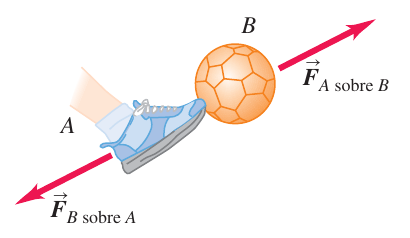
\includegraphics[scale=0.8]{img/2.5-1.png}
    \end{figure}

    \par Expresando en palabras, en la tercera ley de Newton, "acción" y "reacción" son las dos fuerzas opuestas, y Podemos llamarlas \bl{Par acción-reacción}.

    \newsubsection{Diagramas de cuerpo libre}

    \par En esta sección mencionaremos algunas ideas y técnicas que Pueden usarse en cualquier problema en que intervengan las leves de Newton.

    \begin{enumerate}
        \item Las leves de Newton se aplican a un cuerpo específico. Siempre tenés que definir que cuerpo vas a analizar.
        \item En la sumatoria de fuerzas F, solo se incluyen las fuerzas que actúan sobre el cuerpo, no las que el cuerpo ejerce sobre otros. Si analizás a una persona caminando, incluís la fuerzas del suelo sobre la persona, no la que la persona ejerce sobre el suelo.
        \item Un diagrama de cuerpo libre muestra el cuerpo aislado con todas las fuerzas externas que actúan sobre el, sin incluir fuerzas que el cuerpo ejerce sobre otros.
    \end{enumerate}

    \begin{figure}[H]
        \centering
        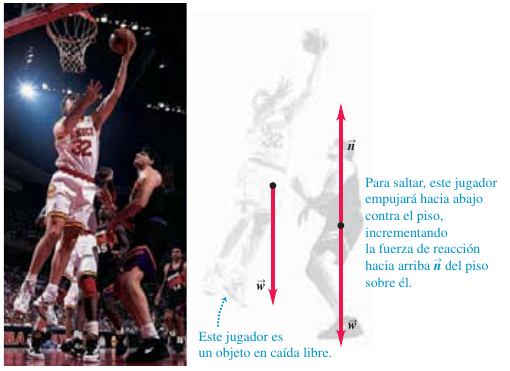
\includegraphics[scale=0.7]{img/2.6-1.png}
    \end{figure}

\newsection{Aplicación de las leyes de Newton}

\par Este capítulo se enfoca en \bl{aplicar las leyes de Newton} a distintos tipos de situaciones reales, como un velero deslizándose sobre hielo, un trineo bajando una colina y un avión dando una vuelta cerrada. A pesar de que las \bl{leyes de Newton} son simples en su formulación, resolver problemas concretos requiere una buena dosis de análisis y técnica.

    \newsubsection{Empleo de la primera ley de Newton: Partículas en equilibrio}

    \par El principio físico fundamental es la primera ley de Newton: si una partícula está en reposo o se mueve con velocidad constante en un marco de referencia inercial, la fuerza neta que actúa sobre ella, es decir, la suma vectorial de todas las fuerzas que actúan sobre ella debe ser cero:

    \definicion{
        \centering
        \par $\Sigma \vec{F} = 0 \quad$ (partícula en equilibrio, forma vectorial)
    }

    \par Esta sección trata sobre el uso de la primera ley de Newton para resolver problemas de cuerpos en equilibrio. Quizás algunos de los problemas parezcan complicados; no obstante, lo importante es recordar que todos los problemas que implican partículas en equilibrio se resuelven igual.

    \newex{Ejercicio 1. Equilibrio unidimensional: Tensión en una cuerda sin masa}

    \par Una gimnasta de masa $m_G = 50.0 kg$ se cuelga del extremo inferior de una cuerda colgante. El extremo superior está fijo al techo de un gimnasio. Suponga que la masa de la cuerda es despreciable.
    \begin{enumerate}
        \item ¿Cuánto pesa la gimnasta?
        \item ¿Qué fuerza (magnitud y dirección) ejerce la cuerda sobre ella?
        \item ¿Qué tensión hay en la parte superior de la cuerda?
    \end{enumerate}
    
    \newex{Solución 1.}

    \par Primero identificamos que la gimnasta y la cuerda, ambos estan en equilibrio. Tenemos como incognita el peso de la gimnasta $w_G$. La cuerda tira de la gimnasta con una fuerza $T_{CG}$ y la gimnasta tira de la cuerda con una fuerza $T_{GC}$. El techo ejerce otra fuerza sobre la cuerda, $T_{TC}$, que provoca que la cuerda y la gimnasta esten en equilibrio.

    \begin{figure}[H]
        \centering
        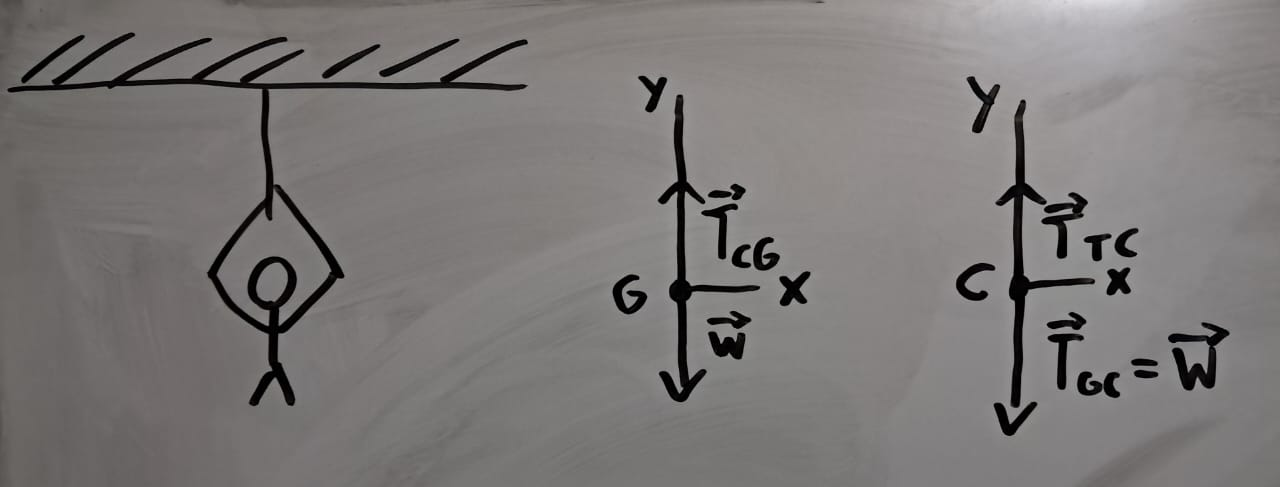
\includegraphics[width=\textwidth]{img/3.1-1.png}
    \end{figure}

    \par El primer digrama representa la situación en si. El segundo diagrama representa las fuerzas que actúan sobre la gimnasta. El tercer diagrama representa las fuerzas que actúan sobre la cuerda.

    \quad

    \par Para calcular el peso de la gimnasta ($\vec{w}$), usaremos la ecuación de la gravedad, derivada de la segunda ley de Newton:

    \[ \lvert \vec{w} \rvert = m \cdot 9.8 \text{m/s}^2 \]
    \[ w_G = 50 \text{kg} \cdot 9.8 \text{m/s}^2 \]
    \[ w_G = 490 \text{N} \]

    \begin{center}
        \par \bl{El peso de la gimnasta es de 490 Newtons}.
    \end{center}

    \par Entonce la magnitud de la fuerza que ejerce la cuerda sobre la gimnasta es: $T_{CG} = 490 \text{N}$. Y su dirección es contraria a la del peso de la gimnasta.

    \par Por el par acción-reacción, existe la fuerza $\vec{T}_{GC} = - \vec{T}_{CG} = \vec{w}$, entonces la gimnasta tira de la cuerda con una fuerza de 490 Newtons con una dirección que apunta hacia abajo. Entonces la fuerza $\vec{T}_{TC}$ es igual en magnitud a $\vec{T}_{GC}$ pero con dirección opuesta, es decir, $\vec{T}_{TC} = - \vec{T}_{GC}$.

    \quad

    \par La \bl{tensión de la cuerda} es de $T_{TC} = 490 \text{N}$ en la parte superior de la cuerda y de $T_{CG} = 490 \text{N}$ en la parte inferior de la cuerda.

    \newsubsection{Empleo de la segunda ley de Newton: Dinámica de partículas}

    \par Ahora podemos analizar problemas de dinámica, donde aplicamos la segunda ley de Newton a cuerpos sobre los cuales la fuerza neta no es cero, de manera que los cuerpos no están en equilibrio sino que tienen aceleración.

    \definicion{
        \centering
        \( \Sigma \vec{F} = m \vec{a} \)
    }

    \newex{Ejercicio 2. Movimiento rectilíneo con una fuerza constante}

    \par Un velero para hielo descansa en una superficie horizontal sin fricción (figura 5.7a). Sopla un viento constante (en la dirección de los patines del trineo), de modo que 4.0 s después de soltarse el velero adquiere una velocidad de 6.0 m>s (unos 22 km/h o 13 mi/h). ¿Qué fuerza constante $F_w$ ejerce el viento sobre el velero? La masa total del velero más el tripulante es de 200 kg.

    \newex{Solución 2.}

    \par Identificamos las variables que se nos dan:

    \begin{itemize}
        \item $m = 200 \text{kg}$
        \item $v(0s) = 0.0 \text{m/s}$
        \item $v(4s) = 22.0 \text{km/h} = 6.1 \text{m/s}$
    \end{itemize}

    \par Para calcular la fuerza usaremos la segunda ley de Newton: $\Sigma \vec{F} = m \vec{a}$. Pero primero debemos calcular la aceleración. Como tenemos una velocidad incial y otra 4s despues podemos utilizar:
    \[ a = \frac{v_1 - v_0}{t_1 - t_0} \]

    \[ a = \frac{6.1 \text{m/s} - 0.0 \text{m/s}}{4.0 \text{s}} = 1.525 \text{m/s}^2 \]

    \par Por lo tanto, la fuerza constante que ejerce el viento sobre el velero es de $F_w = 200 \text{kg} \cdot 1.525 \text{m/s}^2 = 305 \text{N}$

    \newtitle{Peso aparente e ingravidez aparente}

    \par Cuando un pasajero de masa m viaja en un elevador con aceleración ay , una báscula da como peso aparente del pasajero:

    \[ w = m \cdot (g + a_y) \]

    \par Cuando el elevador está acelerando hacia arriba, $a_y$ es positiva y $n$ es mayor que el peso del pasajero $w = mg$. Si el elevador acelera hacia abajo, ay es negativa y n es menor que el peso. Si el pasajero no sabe que el elevador está acelerando, sentirá que su peso cambia y, de hecho, la báscula lo indica. El caso extremo sucede cuando el elevador tiene una aceleración hacia abajo $a_y = -g$, es decir, cuando está en caída libre. En este caso, $n = 0$ y el pasajero siente que no tiene peso.

    \newex{Ejercicio 3. Aceleración cuesta abajo}

    \par Un trineo cargado de estudiantes en vacaciones (peso total $w$) se desliza hacia abajo por una larga cuesta nevada. La pendiente tiene un ángulo constante $\alpha$, y el trineo está tan bien encerado que la fricción es despreciable. ¿Qué aceleración tiene el trineo?

    \newex{Solución 3.}

    \par Necesitamos averiguar la aceleración $a$. Sabemos que la unica fuerza que actua sobre el trineo es la gravedad, y que su peso es $w$.

    \par Para mayor comodidad dibujaremos un diagrama de cuerpo libre inclinado para que el eje x se paralelo a la aceleración $a$, ahora $a_x$.

    \begin{figure}[H]
        \centering
        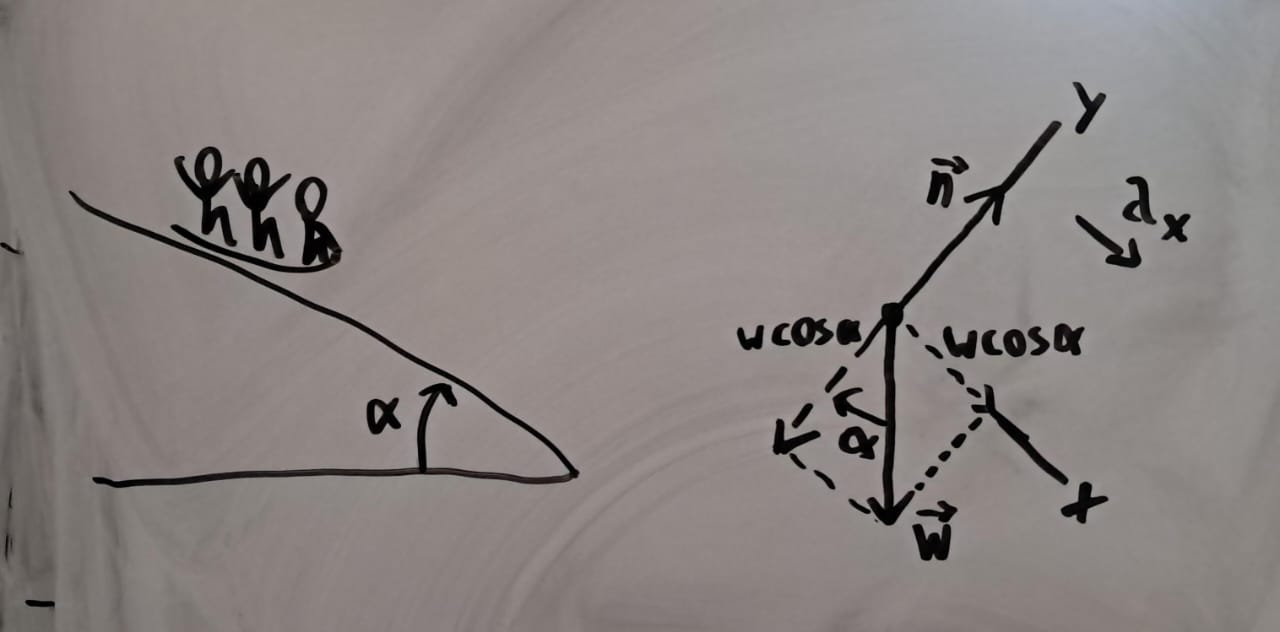
\includegraphics[width=\textwidth]{img/3.2-2.png}
    \end{figure}

    \par Por segunda ley de Newton dividida en componentes tenemos:

    \[ \Sigma F_x = m a_x \]

    \[ \Sigma F_y = m a_y \]

    \par Si sumamos las fuerzas:

    \[ \Sigma F_y = w\cos(\alpha) + (-w\cos(\alpha)) = 0 = m a_y \quad \Longrightarrow  \quad a_y = 0 \]

    \[ \Sigma F_x = w\sin(\alpha) = m a_x \]

    \par Como $w = m g$, tenemos que $\cancel{m} a_x = \cancel{m} g \sin(\alpha)$, dejando como resultado:

    \[ a_x = g \sin(\alpha) \]

    \newsubsection{Fuerzas de fricción}

    \par Hemos visto varios problemas en que un cuerpo descansa o se desliza sobre una superficie que ejerce fuerzas sobre el cuerpo. En esta sección, veremos con detenimiento la fuerza de fricción.

    \par Una fuerza importante en muchos aspectos de nuestra vida es la fricción. El aceite de un motor automotriz reduce la fricción entre piezas móviles; no obstante, sin fricción entre los neumáticos y el asfalto, el automóvil no podría avanzar ni dar vuelta.

    \newtitle{Fricción cinética y estática}

    \begin{multicols}{2}
        \par Primero, cuando un cuerpo descansa o se desliza sobre una superficie, podemos representar la fuerza de contacto que la superficie ejerce sobre el cuerpo en términos de componentes de fuerza perpendiculares y paralelos a la superficie (figura). El vector componente paralelo a la superficie (y perpendicualr a n ) es la fuerza de fricción, denotada con $\vec{f}$. La dirección de la fuerza de fricción siempre es opuesta al movimiento relativo de las dos superficies.

        \begin{figure}[H]
            \centering
            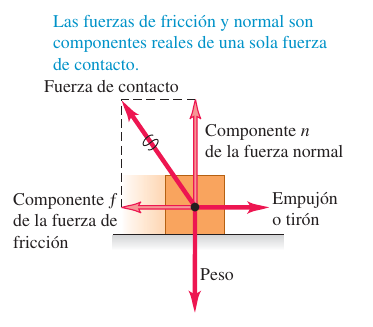
\includegraphics[scale=0.6]{img/3.3-1.png}
        \end{figure}
    \end{multicols}

    \par El tipo de fricción que actúa cuando un cuerpo se desliza sobre una superficie es la \bl{fuerza de fricción cinética $\vec{f}_k$}. La magnitud de esta fuerza suele aumentar al aumentar la fuerza normal. En muchos casos, la magnitud de la fuerza de fricción cinética $f_k$ experimental es aproximadamente proporcional a la magnitud n de la fuerza normal. En tales casos, representamos la relación con la ecuación:

    \definicion{
        \centering
        \par \( f_k = \mu_k \cdot n \) \quad \quad \quad (magnitud de la fuerza de fricción cinética)
    }

    \par donde $\mu_k$ es una constante llamada coeficiente de fricción cinética. Cuanto más resbalosa sea una superficie, menor será el coeficiente de fricción. Al ser el cociente de dos magnitudes de fuerza ($\frac{{f}_k}{{n}}$), $\mu_k$ es un número puro sin unidades. (Caso similar a la masa inercial).

    \vspace{0.5cm}

    \par \color{red} \underline{DISCLAIMER}: \color{black} La ecuación sólo es una representación aproximada de un fenómeno complejo. En el nivel microscópico, las fuerzas de fricción y la normal se deben a las fuerzas intermoleculares (fundamentalmente eléctricas) entre dos superficies ásperas en los puntos donde entran en contacto.

    \vspace{0.5cm}

    \par Las fuerzas de fricción también pueden actuar cuando no hay movimiento relativo. Si tratamos de deslizar por el piso una caja con libros, tal vez no se mueva porque el piso ejerce una fuerza de fricción igual y opuesta sobre la caja. Ésta se llama \bl{fuerza de fricción estática $\vec{f}_s$}.

    \begin{figure}[H]
        \centering
        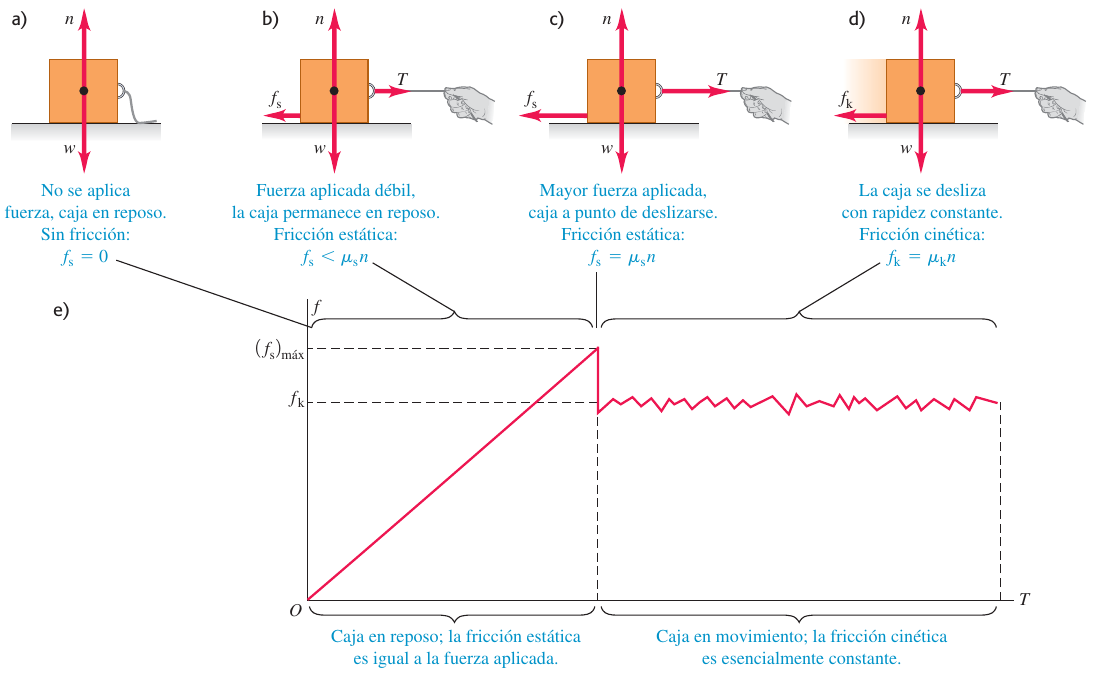
\includegraphics[width=\textwidth]{img/3.3-2.png}
    \end{figure}

    \begin{center}
        \par \bl{Tabla: Coeficientes de fricción aproximados}
    \end{center}

    \begin{table}[H]
        \centering
        \begin{tabular}{|c|c|c|}
            \hline
            Materiales & Coeficiente de fricción estática, $\mu_s$ & Coeficiente de fricción cinética, $\mu_k$ \\
            \hline
            Acero sobre acero & 0.74 &  0.57 \\
            \hline
            Aluminio sobre acero & 0.61 &  0.47 \\
            \hline
            Cobre sobre acero & 0.53 &  0.36 \\
            \hline
            Latón sobre acero & 0.51 &  0.44 \\
            \hline
            Zinc sobre hierro colado & 0.85 &  0.21  \\
            \hline
            Cobre sobre hierro colado & 1.05 &  0.29  \\
            \hline
            Vidrio sobre vidrio & 0.94 &  0.40  \\
            \hline
            Cobre sobre vidrio & 0.68  &  0.53  \\
            \hline
            Teflón sobre teflón & 0.04 &  0.04 \\
            \hline
            Teflón sobre acero & 0.04 &  0.04 \\
            \hline
        \end{tabular}
    \end{table}

    \newex{Ejercicio 4. Fricción en movimiento horizontal}

    \par Usted intenta mover una caja de $500N$ por un piso horizontal. Para comenzar a moverla, debe tirar con una fuerza horizontal de $230N$. Una vez que la caja “se libera” y comienza a moverse, puede mantenerse a velocidad constante con sólo $200N$. ¿Cuáles son los coeficientes de fricción estática y cinética?

    \newex{Solución 4.}

    \par Sabemos que la caja esta en reposo cuando se le aplica una fuerza de $230N$ en el eje x.

    \begin{figure}[H]
        \centering
        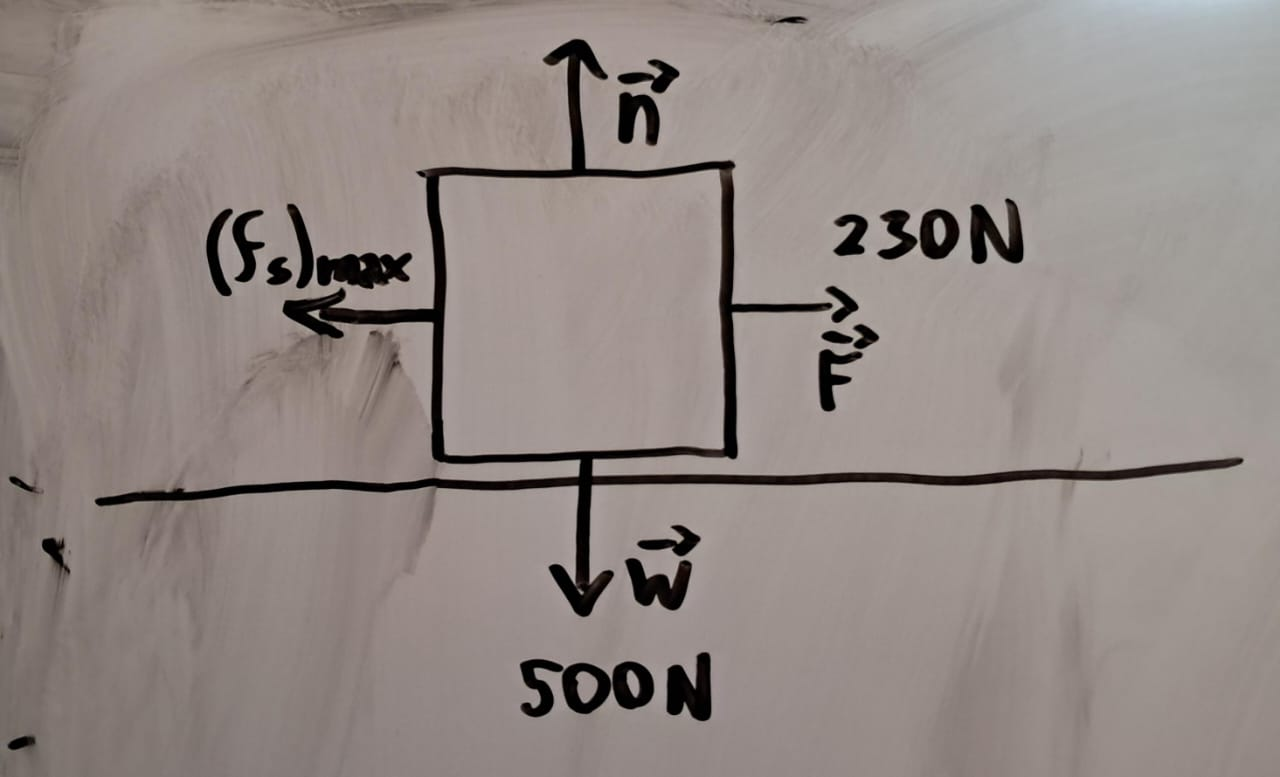
\includegraphics[width=0.5\textwidth]{img/3.3-3.png}
    \end{figure}

    \par Usando la primera ley de Newton por componentes tenemos:

    \[ \Sigma F_x = n + (-w) = 0 \quad \Longrightarrow \quad n = w = 500N \]

    \[ \Sigma F_y = F + (-(f_s)_{max}) = 0 \quad \Longrightarrow \quad F = (f_s)_{max} = 230N \]

    \par Entonces podemos calcular el coeficiente de fricción estática:

    \[ \mu_s = \frac{F}{n} = \frac{230N}{500N} = 0.46 \]

    \par También sabemos que si la caja esta en movimiento horizontal se mantendra en equilibrio si se le aplica una fuerza de $200N$:

    \begin{figure}[H]
        \centering
        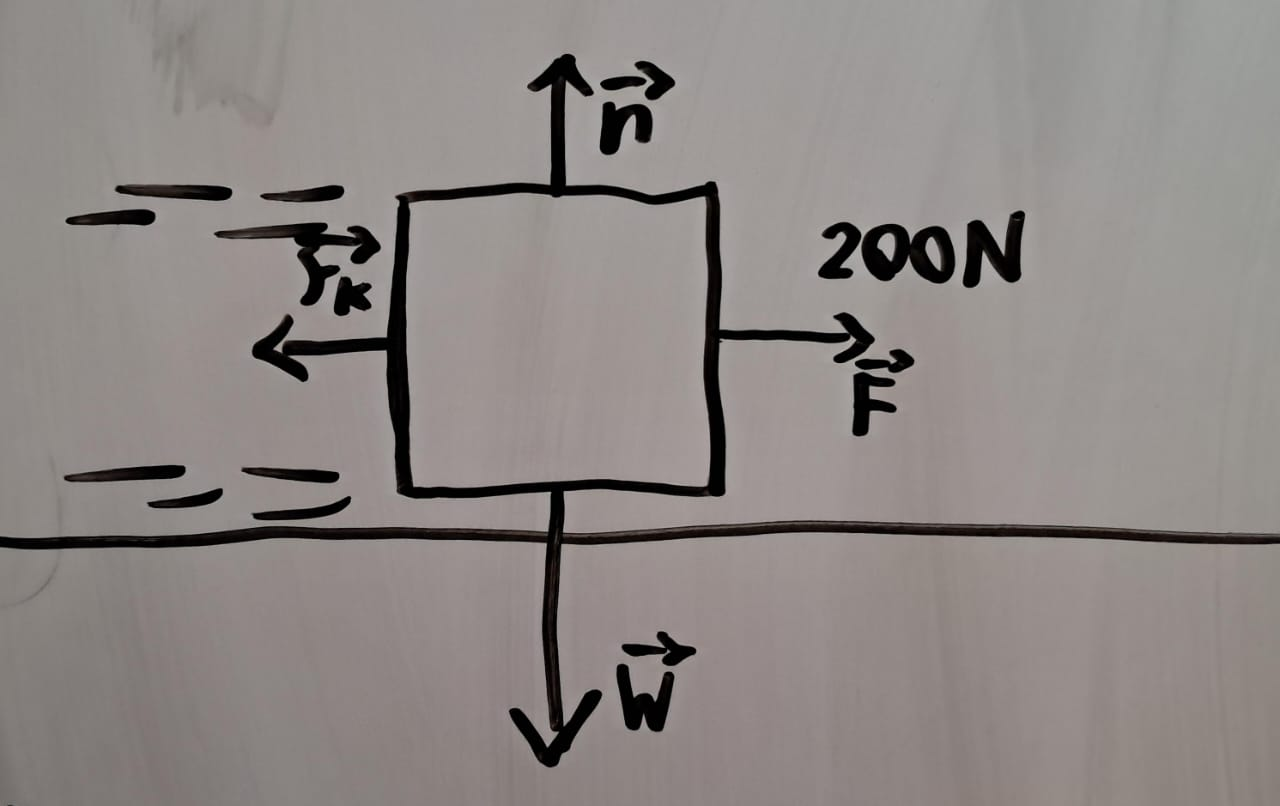
\includegraphics[width=0.5\textwidth]{img/3.3-4.png}
    \end{figure}

    \par Usando la primera ley de Newton por componentes tenemos:

    \[ \Sigma F_x = n + (-w) = 0 \quad \Longrightarrow \quad n = w = 500N \]

    \[ \Sigma F_y = F + (-f_k) = 0 \quad \Longrightarrow \quad F = f_k = 200N \]

    \par Entonces podemos calcular el coeficiente de fricción cinética:

    \[ \mu_k = \frac{F}{n} = \frac{200N}{500N} = 0.4 \]

    \par Concluimos que el coeficiente de fricción estática es $0.46$ y el coeficiente de fricción cinética es $0.4$.

    \newex{Ejercicio 5. Reducción al mínimo de la fricción cinética}

    \par En el ejercicio anterior, suponga que usted intenta mover la caja atando una cuerda a ella y tira de la cuerda hacia arriba con un ángulo de 30° sobre la horizontal. ¿Qué fuerza debe aplicar al tirar para mantener la caja en movimiento con velocidad constante? ¿Esto es más fácil o difícil que tirar horizontalmente? Suponga que $w = 500N$ y $\mu_k = 0.40$.

    \newex{Solución 5.}

    \par Sabemos que la caja esta en equilibrio (su velocidad es constante) entonces aplicamos la primera ley de Newton para encontrar la fuerza $T$ que se debe aplicar para mantener la caja en movimiento:

    \par Primero hacemos un diagrama de cuerpo libre:

    \begin{figure}[H]
        \centering
        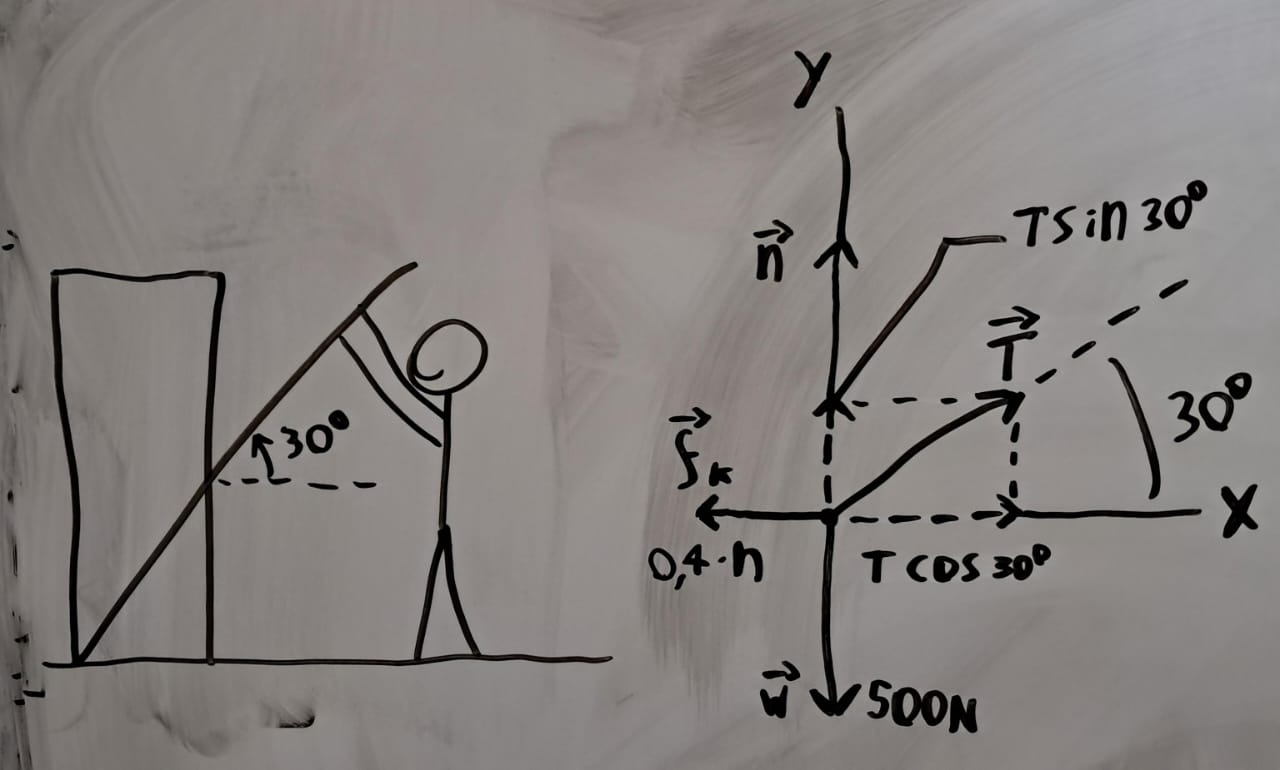
\includegraphics[width=0.8\textwidth]{img/3.3-5.png}
    \end{figure}

    \par Usando la primera ley de Newton por componentes tenemos:

    \[ \Sigma F_x = T\cos(30^\circ) + (-f_k) = 0 \quad \Longrightarrow \quad T\cos(30^\circ) = f_k \]

    \[ \Sigma F_y = T\sin(30^\circ) + n + (-w) = 0 \quad \Longrightarrow \quad n = w - T\sin(30^\circ) \]

    \vspace{0.5cm}

    \par Para encontrar la fuerza $T$ tenemos que usar el hecho de que $f_k = T\cos(30^\circ)$:

    \[ T\cos(30^\circ) = f_k = \mu_k \cdot n \]

    \par Remplazando:

    \[ T\cos(30^\circ) = \mu_k \cdot (w - T\sin(30^\circ)) \]

    \par Despejando $T$ tenemos:

    \[ T = \frac{\mu_k \cdot w}{cos(30^\circ) + \mu_k \sin(30^\circ)} = \frac{0.40 \cdot 500N}{cos(30^\circ) + 0.40 \sin(30^\circ)} \approx 188N \]

    \vspace{0.5cm}

    \par Concluimos que la fuerza $T$ que debe aplicar para mantener la caja en movimiento es de 188N.

    \vspace{0.5cm}

    \par Por otro lado, si se intenta mover la caja horizontalmente, entonces la fuerza $T$ que se debe aplicar para mantener la caja en movimiento es de $\mu_k \cdot n = 0.40 \cdot 500N = 200N$. Al no ser reducida la fuerza normal $f_k$ no se reduce por lo que la fricción "jode" más al tratar de mover la caja.

    \newtitle{Fricción de rodamiento}

    \par Es mucho más fácil mover un archivero lleno de documentos sobre un piso horizontal usando un carrito con ruedas que deslizándolo. Podemos definir un \bl{coeficiente de fricción de rodamiento $\mu_r$}, que es la fuerza horizontal necesaria para lograr rapidez constante en una superficie plana, dividida entre la fuerza normal hacia arriba ejercida por la superficie. Cuyo valor suele ser de 0.002 a 0.003 para ruedas de acero sobre rieles de acero, y de 0.01 a 0.02 para ruedas de caucho sobre concreto.

    \newex{Ejercicio 6. Movimiento con fricción de rodamiento}

    \par ...

    \newtitle{Resistencia de fluidos y rapidez terminal}

    \par Si usted saca la mano por la ventanilla de un automóvil que viaja con gran rapidez, comprobará la existencia de la \bl{resistencia de un fluido}, que es la fuerza que un fluido (gas o líquido) ejerce sobre un cuerpo que se mueve a través de él.

    \par La dirección de la fuerza de resistencia de un fluido que actúa sobre un cuerpo siempre es opuesta a la dirección de la velocidad del cuerpo. La magnitud de la fuerza de resistencia de un fluido suele aumentar al incrementarse la rapidez del cuerpo en el fluido. Esto es muy diferente de la fuerza de fricción cinética entre dos superficies en contacto, que casi siempre podemos considerar independiente de la rapidez. A rapidez baja, la magnitud f de la fuerza de resistencia del fluido es aproximadamente proporcional a la rapidez $v$ del cuerpo:

    \definicion{ 
        \centering
        $f = k v$ \quad \quad (resistencia del fluido a baja rapidez)
        }

    
    \noindent donde $k$ es una constante de proporcionalidad que depende de la forma y el tamaño del cuerpo, y las propiedades del fluido. Las unidades de este $k$ son $ [k] = \frac{N}{m/s} = \frac{kg \cdot \frac{m}{s^2} \cdot s }{m} = \frac{kg}{s}$.

    \par La fuerza de resistencia es aproximadamente proporcional a $v^2$, no a $v$, para la rapidez de una pelota de tenis o una rapidez mayor y se denomina \bl{arrastre del aire} o sólo arrastre. En este caso, sustituimos la ecuación por la siguiente:

    \definicion{
        \centering
        $f = D v^2$ \quad \quad (resistencia de fluidos a alta rapidez)
    }

    \par Por la dependencia de $v^2$, el arrastre aumenta rápidamente conforme se incrementa la rapidez. Las unidades de este $D$ son $ [D] = \frac{N}{m^2/s^2} = \frac{kg \cdot \frac{m}{s^2} \cdot s^2 }{m^2} = \frac{kg}{m}$.

    \vspace{0.5cm}

    \par Por los efectos de la resistencia de fluidos, un objeto que cae en un fluido no tiene aceleración constante. Para describir su movimiento debemos partir de la segunda ley de Newton.

    \vspace{2cm}

    \begin{multicols}{2}
        \begin{minipage}{0.6\textwidth}
            \par Consideremos esta situación: suponga que usted suelta una roca en la superficie de un estanque profundo, y cae hasta el fondo (figura). En este caso, la fuerza de resistencia del fluido está dada por la ecuación de resistencia del fluido a baja rapidez. ¿Cómo cambian la aceleración, velocidad y posición de la roca con el tiempo?
            
        \end{minipage}

        \columnbreak

        \begin{minipage}{0.6\textwidth}
            \centering

            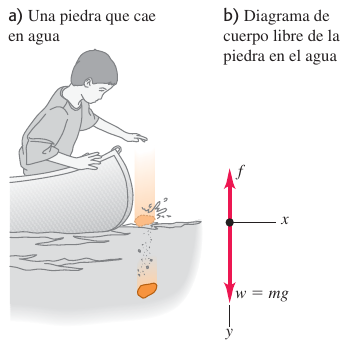
\includegraphics[width=0.6\textwidth]{img/3.3-6.png}
        \end{minipage}
    \end{multicols}

    \par Si observamos el diagrama de cuerpo libre podemos ver que $\Sigma F_x = 0$ entonces solo tomamos en cuenta la componente $y$:

    \[ \Sigma F_y = mg + (-f) = mg + (-kv_y) = ma_y \]

    \par Al principio, cuando la roca empieza a moverse, $v_y = 0$, la fuerza de resistencia es cero y la aceleración inicial es $a_y = g$. Al aumentar la rapidez, también se incrementa la fuerza de resistencia hasta ser igual en magnitud al peso. Ahora, $mg - kv_y = 0$, la aceleración se vuelve cero y ya no aumenta la rapidez. A esta rapidez final $v_t$, se le llama \bl{rapidez terminal}, y esta dada por $mg - kv_t = 0$, es decir:

    \[ v_t = \frac{mg}{k} \quad \quad \text{(\bl{rapidez terminal})} \]

    \par La siguiente figura muestra cómo varían la aceleración, la velocidad y la posición con el tiempo.

    \begin{figure}[H]
        \centering
        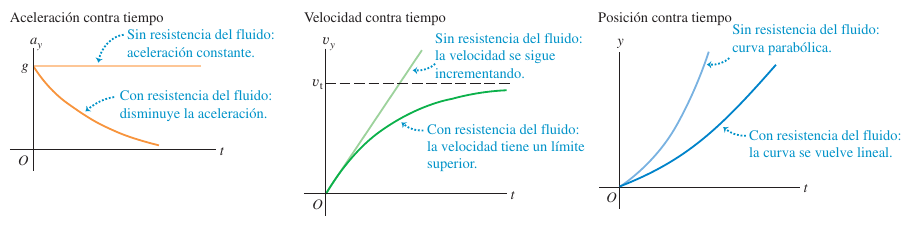
\includegraphics[width=\textwidth]{img/3.3-7.png}
    \end{figure}

    \newsubsection{Dinámica del movimiento circular}

    \par Cuando una partícula se mueve en un círculo con rapidez constante, su aceleración siempre es hacia el centro del círculo (perpendicular a la velocidad instantánea). La magnitud $a_{rad}$ de la aceleración es constante y está dada en términos de la rapidez $v$ y el radio $R$ del círculo por

    \definicion{
        \centering
        \( a_{rad} = \frac{v^2}{R} \) \quad \quad (movimiento circular uniforme)
    }

    \par El subíndice “$rad$” nos recuerda que en cada punto la aceleración siempre es radial hacia el centro del círculo, perpendicular a la velocidad instantánea. Se le denomina \bl{aceleración centrípeta}.

    \vspace{0.5cm}

    \begin{multicols}{2}

        \begin{minipage}{0.5\textwidth}
            \par El movimiento circular uniforme, como todos los movimientos de una partícula, se rige por la segunda ley de Newton. Para hacer que la partícula acelere hacia el centro del círculo, la fuerza neta $\Sigma \vec{F}$ sobre la partícula debe estar dirigida siempre hacia el centro. La magnitud de la aceleración es constante, así que la magnitud $F_{net}$ de la fuerza neta también debe ser constante. Si deja de actuar la fuerza neta hacia adentro, la partícula saldrá disparada en una línea recta tangente al círculo (ver figura).
        \end{minipage}

        \columnbreak

        \begin{minipage}{0.5\textwidth}
            \centering
            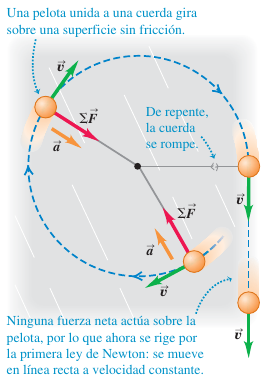
\includegraphics[width=0.7\textwidth]{img/3.3-8.png}
        \end{minipage}

    \end{multicols}

    \par ...


    \newsubsection{Fuerzas fundamentales de la naturaleza}

    \par Hemos visto fuerzas de varios tipos —peso, tensión, fricción, resistencia de fluidos y la fuerza normal— y veremos otras más al seguir estudiando física. Pero, ¿cuántas clases distintas de fuerzas hay? Actualmente, se considera que todas las fuerzas son expresiones de tan sólo cuatro clases de fuerzas o interacciones fundamentales entre las partículas.

    \begin{multicols}{2}

        \begin{minipage}{0.6\textwidth}

            \par Las \bl{interacciones gravitacionales} incluyen la fuerza familiar del peso, que se debe a la acción de la atracción gravitacional terrestre sobre un cuerpo. La mutua atracción gravitacional entre las diferentes partes de la Tierra mantienen a nuestro planeta unido (figura a).

            \vspace{0.2cm}

            \par Las \bl{interacciones electromagnéticas}, incluye las fuerzas eléctricas y magnéticas. Si nos frotamos un peine por el cabello, al final el peine tendrá una carga eléctrica; es posible usar la fuerza eléctrica para atraer trocitos de papel. Todos los átomos contienen carga eléctrica positiva y negativa, así que átomos y moléculas pueden ejercer fuerzas eléctricas unos sobre otros (figura b).

            \vspace{0.2cm}

            \par Las otras dos clases de interacciones son menos conocidas. La \bl{interacción fuerte} mantiene unido el núcleo de un átomo. Los núcleos contienen neutrones (eléctricamente neutros) y protones (con carga positiva). La fuerza eléctrica entre protones hace que se repelan mutuamente; la enorme fuerza de atracción entre las partículas nucleares contrarresta esta repulsión y mantiene el núcleo estable. En este contexto, la interacción fuerte también se denomina fuerza nuclear fuerte; tiene un alcance mucho menor que las interacciones eléctricas, pero es mucho más fuerte dentro de ese alcance. La interacción fuerte juega un papel fundamental en las reacciones termonucleares que ocurren en el núcleo del Sol, y que generan el calor y su luz (figura c).

            \vspace{0.2cm}

            \par Por último, tenemos la \bl{interacción débil} cuyo alcance es tan pequeño que es relevante sólo a una escala de núcleo o menor. La interacción débil causa una forma común de radioactividad, llamada desintegración beta, en la que un neutrón de un núcleo radioactivo se transforma en protón al tiempo que expulsa un electrón y una partícula casi sin masa llamada antineutrino electrónico. La interacción débil entre un antineutrino y la materia ordinaria es tan tenue que el antineutrino fácilmente podría atravesar una pared de plomo ¡de un millón de kilómetros de espesor! Incluso cuando una estrella gigante sufrió una explosión cataclísmica llamada supernova, la mayoría de la energía fue liberada mediante la interacción débil (figura d).

        \end{minipage}

        \columnbreak

        \begin{minipage}{0.6\textwidth}
            \centering
            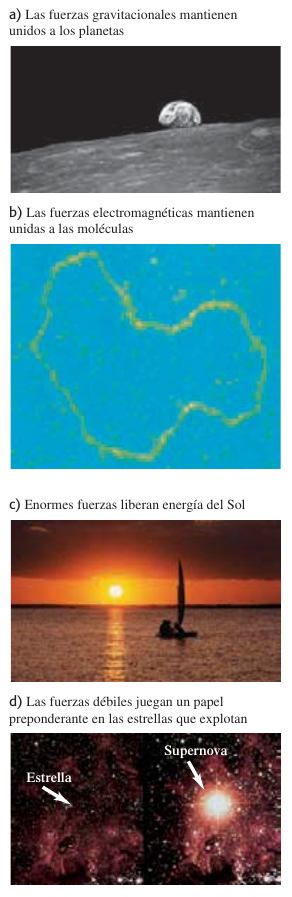
\includegraphics[width=0.6\textwidth]{img/3.3-9.png}
        \end{minipage}
    \end{multicols}

    \vspace{2cm}

    \newsection{Trabajo y Energía Cinética}

    \par En este capítulo nos concentraremos en la mecánica. Conoceremos una importante forma de energía, la energía cinética o la energía de movimiento, y su relación con el concepto de trabajo. También consideraremos la potencia, que es la rapidez con que se realiza trabajo.

    \newsubsection{Trabajo}

    \par En esta sección aprenderemos cómo se define el trabajo y cómo se calcula en diversas situaciones que implican fuerzas constantes. Aunque ya sabemos cómo resolver problemas donde las fuerzas son constantes, el concepto de trabajo nos resultará útil. Más adelante en este capítulo deduciremos la relación entre trabajo y energía cinética, y la aplicaremos después en problemas donde las fuerzas no son constantes.

    \par Estos tres ejemplos de trabajo —mover un sofá, levantar una pila libros y empujar un automóvil— tienen algo en común. En ellos realizamos trabajo ejerciendo una fuerza sobre un cuerpo mientras éste se mueve de un lugar a otro, es decir, sufre un desplazamiento. Efectuamos más trabajo si la fuerza es mayor (empujamos más fuerte el auto) o si el desplazamiento es mayor (lo empujamos una mayor distancia).

    \par El físico define el trabajo con base en estas observaciones. Considere un cuerpo que sufre un desplazamiento de magnitud $s$ en línea recta. (Por ahora, supondremos que todo cuerpo puede tratarse como partícula y despreciaremos cualquier rotación o cambio en la forma del cuerpo.) Mientras el cuerpo se mueve, una fuerza constante $\vec{F}$ actúa sobre él en la dirección del desplazamiento $\vec{s}$. Definimos el trabajo $W$ realizado por esta fuerza constante en dichas condiciones como el producto de la magnitud $F$ de la fuerza y la magnitud $s$ del desplazamiento:

    \definicion{
        \centering
        \(W = Fs\) \text{(fuerza constante en dirección del desplazamiento rectilíneo)}
    }

    \par La unidad de trabajo en el SI es el joule (que se abrevia $J$ y se pronuncia “yul”,nombrada así en honor del físico inglés del siglo XIX James Prescott Joule). En el SI la unidad de fuerza es el newton y la unidad de distancia es el metro, así que 1 joule equivale a un new-ton-metro ($N \cdot m$):

    \[1 J = 1 N \cdot m\]

    \par En el sistema británico, la unidad de fuerza es la libra (Ib), la unidad de distancia es el pie (ft), y la unidad de trabajo es el pie-libra ($ft \cdot Ib$). Estas conversiones son útiles:

    \[1 J =  0.7376 ft \cdot 1Ib \quad \quad  1 ft \cdot lb = 1.356 J\]

    \vspace{0.5cm}

    \par Pensemos en una persona que empuja un automóvil averiado. Si lo empuja a lo largo de un desplazamiento $\vec{s}$ con una fuerza constante $\vec{F}$ en la dirección del movimiento, la cantidad de trabajo que efectúa sobre el auto está dada por la ecuación:$W = Fs$. Sin embargo, ¿y si la persona hubiera empujado con un ángulo $\phi$ con respecto al desplazamiento del auto (figura)?

    \begin{figure}[H]
        \centering
        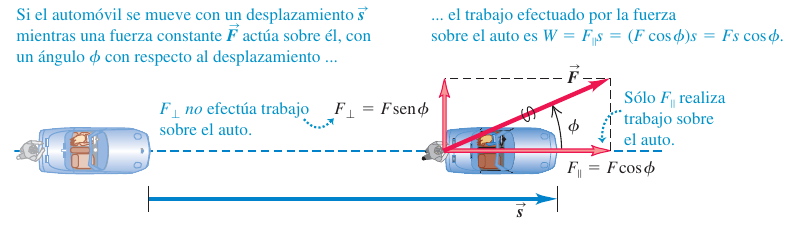
\includegraphics[width=\textwidth]{img/5.1-1.png}
        
    \end{figure}
    
    \par Entonces $\vec{F}$ tiene una componente $F_{\parallel} = F cos \phi$ en la dirección del desplazamiento y una componente $F_{\perp} = F sin \phi$ que actúa perpendicular al desplazamiento.

    \par En este caso, sólo la componente paralela $F_{\parallel}$ es eficaz para mover el auto, por lo que definimos el trabajo como el producto de esta componente de fuerza y la magnitud del desplazamiento. Por lo tanto:

    \[W = Fs cos \phi \]

    \par La ecuación tiene la forma del producto escalar de dos vectores. Ello nos permite escribir la ecuación de forma más compacta:

    \[W = \vec{F} \cdot \vec{s}\]

    \newex{Ejercicio 7. Trabajo efectuado por una fuerza constante}

    \par a) Esteban ejerce una fuerza constante de magnitud $210N$ sobre el automóvil averiado de la figura anterior, mientras lo empuja una distancia de $18m$. Además, un neumático se desinfló, así que, para lograr que el auto avance al frente, Esteban debe empujarlo con un ángulo de $30^\circ$ con respecto a la dirección del movimiento. ¿Cuánto trabajo efectúa Esteban?

    \par b) Con ánimo de ayudar, Esteban empuja un segundo automóvil averiado con una fuerza constante $\vec{F} = (160N)\hat{i} - (40N)\hat{j}$. El desplazamiento del automóvil es $\vec{s} = (14m)\hat{i} + (11m)\hat{j}$ ¿Cuánto trabajo efectúa Esteban en este caso?

    \newex{Solución 7.}

    \par ...

    \newtitle{Trabajo: Positivo, negativo o cero}

    \par En el ejercicio anterior, el trabajo efectuado al empujar los autos fue positivo. No obstante, es importante entender que el trabajo también puede ser negativo o cero. Ésta es la diferencia esencial entre la definición de trabajo en física y la definición “cotidiana” del mismo.

    \begin{figure}[H]
        \centering
        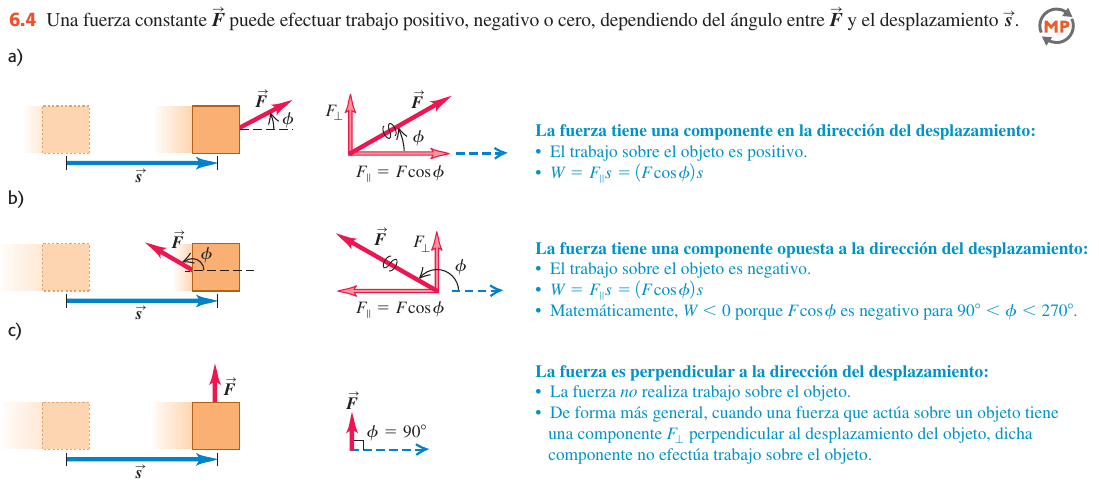
\includegraphics[width=\textwidth]{img/5.1-2.png}
    \end{figure}

    \newtitle{Trabajo total}

    \par ¿Cómo calculamos el trabajo cuando varias fuerzas actúan sobre un cuerpo? Podemos usar las ecuaciones anteriormente vistas para calcular el trabajo realizado por cada fuerza individual. Puesto que el trabajo es una cantidad escalar, el trabajo total $W_{tot}$ realizado por todas las fuerzas sobre el cuerpo es la suma algebraica de los trabajos realizados por las fuerzas individuales. Otra forma de calcular $W_{tot}$ es calcular la suma vectorial de las fuerzas (es decir, la fuerza neta) y usarla en vez de $\vec{F}$.

    \newex{Ejercicio 8. Trabajo realizado por varias fuerzas}

    \par Un granjero engancha su tractor a un trineo cargado con leña y lo arrastra 20 m sobre el suelo horizontal. El peso total del trineo y la carga es de $14700 N$. El tractor ejerce una fuerza constante de $5000 N$ a $36.9^\circ$ sobre la horizontal. Una fuerza de fricción de $3500 N$ se opone al movimiento del trineo. Calcule el trabajo realizado por cada fuerza que actúa sobre el trineo y el trabajo total de todas las fuerzas.

    \newex{Solución 8.}

    \begin{figure}[H]
        \centering
        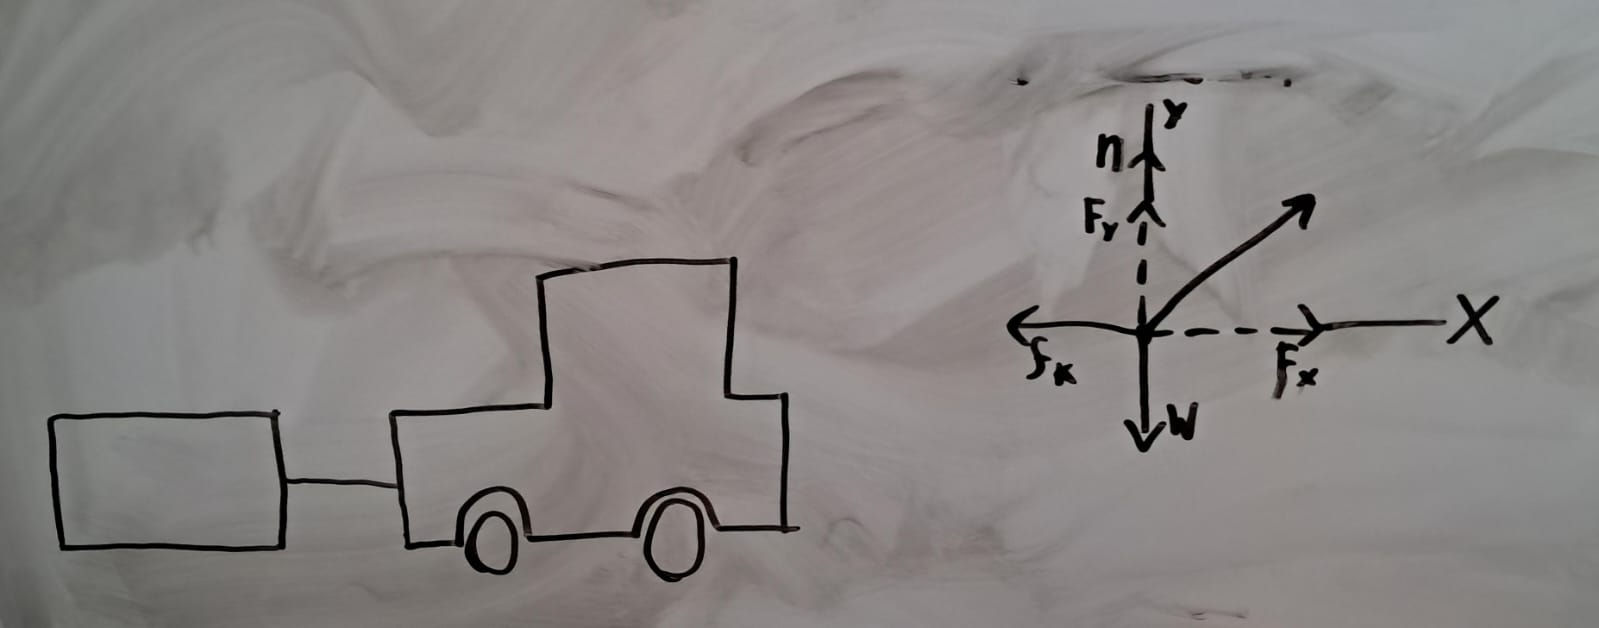
\includegraphics[width=\textwidth]{img/5.1-3.png}
    \end{figure}

    \par ...
    
    \vspace{6cm}

    \newsubsection{Energía cinética y el teorema trabajo-energía}

    \par El trabajo total realizado por fuerzas externas sobre un cuerpo se relaciona con el desplazamiento de éste (los cambios en su posición), pero también está relacionado con los cambios en la rapidez del cuerpo. Para comprobarlo, considere la siguiente figura, que muestra tres ejemplos de un bloque que se desliza sobre una mesa sin fricción. Las fuerzas que actúan sobre el bloque son su peso $\vec{w}$, la fuerza normal $\vec{n}$ y la fuerza $\vec{F}$ ejercida por la mano.

    \begin{figure}[H]
        \centering
        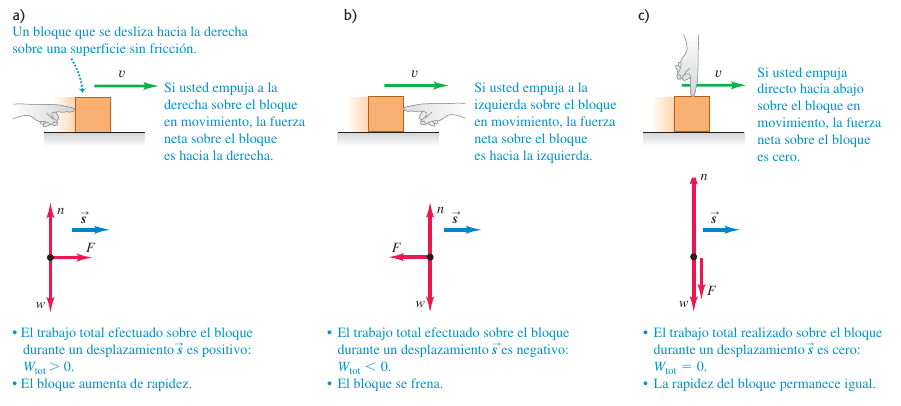
\includegraphics[width=\textwidth]{img/5.2-1.png}
    \end{figure}
    
    \par Hagamos más cuantitativas tales observaciones. Considere una partícula con masa $m$ que se mueve en el eje $x$ bajo la acción de una fuerza neta constante de magnitud $F$ dirigida hacia el eje $+x$ (figura). La aceleración de la partícula es constante y está dada por la segunda ley de Newton, $F = m a_x$. Suponga que la rapidez cambia de $v_1$ a $v_2$ mientras la partícula sufre un desplazamiento $s = x_2 - x_1$ del punto $x_1$ al $x_2$.

    \begin{figure}[H]
        \centering
        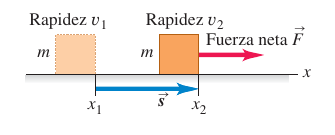
\includegraphics[width=0.5\textwidth]{img/5.2-2.png}
    \end{figure}

    \par Primero buscamos una ecuación que solo relaciona $v$, $a_x$ y $s$ (el desplazamiento). Para ello utilizamos estas ecuaciones de MRUA:

    \[\text{1.}\quad v = v_1 + a_xt\]

    \[\text{1.}\quad x = x_1 + v_1t + \frac{1}{2}a_xt^2\]

    \par Eliminamos el tiempo $t$ (utilizando 1.):

    \[t = \frac{v-v_1}{a_x}\]

    \par Sustituyendo en la ecuación de posición:

    \[s = x - x_1 = v_1 t + \frac{1}{2} a_x t^2\]

    \[s = v_1 \left(\frac{v-v_1}{a_x}\right)  + \frac{1}{2} a_x \left(\frac{v-v_1}{a_x}\right) ^2\]

    \par Multiplicamos y simplificamos:

    \[s = \frac{v_1 (v - v_1)}{a_x} + \frac{(v-v_1)^2}{2 a_x}\]

    \par Multiplicamos todo por $2a_x$

    \[ 2a_x s = 2 v_1 (v - v_1) + (v - v_1)^2 \]

    \par Expandimos:

    \[ 2a_x s = 2 v_1 v - 2 v_1^2 + v^2 - 2 v_1 v + v_1^2\]

    \par Se cancelan los términos $2v_1v - 2v_1v$, y queda:

    \[ 2a_x s = v^2 - v_1^2\]

    \vspace{1cm}

    \par Obeniendo una ecuación para la aceleración en función de la rapidez y el desplazamiento:

    \[ a_x = \frac{v_2^2 - v_1^2}{2s}\]

    \par Al multiplicar esta ecuación por $m$ y sustituir $m a_x$ por la fuerza neta $F$, obtenemos

    \[ F = m a_x = m \frac{v_2^2 - v_1^2}{2s}\]

    \[\text{(5.2-1)} \quad Fs = \frac{1}{2} m v_2^2 - \frac{1}{2} m v_1^2\]

    El producto $Fs$ es el trabajo efectuado por la fuerza neta $F$ y, por lo tanto, es igual al trabajo total $W_{tot}$ efectuado por todas las fuerzas que actúan sobre la partícula. Llamamos a la cantidad $\frac{1}{2}mv^2$ la \bl{energía cinética} $K$ de la partícula (definición de energía cinética):

    \definicion{
        \centering
        \( K = \frac{1}{2}mv^2 \quad \quad \text{(definición de energía cinética)} \)
    }

    \par Igual que el trabajo, la energía cinética de una partícula es una cantidad escalar; sólo depende de la masa y la rapidez de la partícula, no de su dirección de movimiento. Un automóvil (visto como partícula) tiene la misma energía cinética yendo al norte a $10 m/s$ que yendo al este a $10 m/s$. La energía cinética nunca puede ser negativa, y es cero sólo si la partícula está en reposo.

    \par Ahora podemos interpretar la ecuación (5.2-1) en términos de trabajo y energía cinética.

    \definicion{
        \par El trabajo efectuado por la fuerza neta sobre una partícula es igual al cambio de energía cinética de la partícula:
        \[ W_{tot} = K_2 - K_1 = \Delta K \]
    }

    \par Éste es el resultado del \bl{teorema trabajo-energía}.

    \newex{Ejercicio 9. Uso de trabajo y energía para calcular rapidez}

    \par Supongamos que un trineo tiene una rapidez inicial $v_1$ de $2.0 m/s$. ¿Cuál es la rapidez final del trineo después de avanzar 20 m? Con $w = 14700 N$ y $W_{tot} = 10000J$

    \newex{Solución 9.}

    \par Para calcular $v_2$, usaremos el hecho de que $K = \frac{1}{2}m v^2$

    \[ K_2 = W_{tot} + K_1 \]

    \par Para calcular $K_2$, necesitamos calcular $K_1$:

    \[ K_1 = \frac{1}{2} m v_1^2 \]

    \par Para calcularla buscamos el valor de la masa:

    \[ m = \frac{w}{g} = \frac{14700}{9.8} \approx 1430 kg \]

    \par Luego

    \[ K_1 = \frac{1}{2} \cdot 1430 kg \cdot (2.0 m/s)^2 = \frac{1}{2} \cdot 1430 kg \cdot 4.0 m^2/s^2 \approx 2860 J \]

    \par Ahora estamos listos para calcular $K_2$:

    \[ K_2 = W_{tot} + K_1 = 10000 J + 2860 J = 12860 J \Longrightarrow  \]

    \[ \Longrightarrow 12860 J = \frac{1}{2}m v_2^2 \Longrightarrow v_2^2 = \frac{12860 J}{1/2 \cdot 1430 kg} \approx 18 m^2/s^2 \]

    \[ v_2 = \sqrt{18 m^2/s^2} \approx 4.2 m/s \]

\end{document}